\documentclass[17pt,a4paper,landscape]{extarticle}
\usepackage[margin=2.35cm,top=0.12cm,left=1.05cm]{geometry}
\usepackage{amsmath}
\usepackage{amssymb}
\usepackage{tasks}
\usepackage{tikz}
\usepackage{xcolor}
\usepackage[sfdefault,lf]{FiraSans}
\renewcommand{\familydefault}{\sfdefault}
\setlength{\parindent}{0pt}
\pagestyle{empty}
\settasks{label=\textbf{\arabic*.}, label-width=2.2em, item-indent=2.95em, column-sep=2.1cm, after-item-skip=4.7em}
\renewcommand{\arraystretch}{1.15}
\everymath{\displaystyle}

\begin{document}
\sffamily
\boldmath

\boldmath

\boldmath

{\LARGE \textbf{Drawing exponential graphs — Excellence}}\\[0.2em]
Sketch each graph carefully. Mark the horizontal asymptote when asked.

\begin{tasks}(3)
\task {Draw \mbox{$y=2^{x}+4$}. Mark the horizontal asymptote. \\[0.4em] 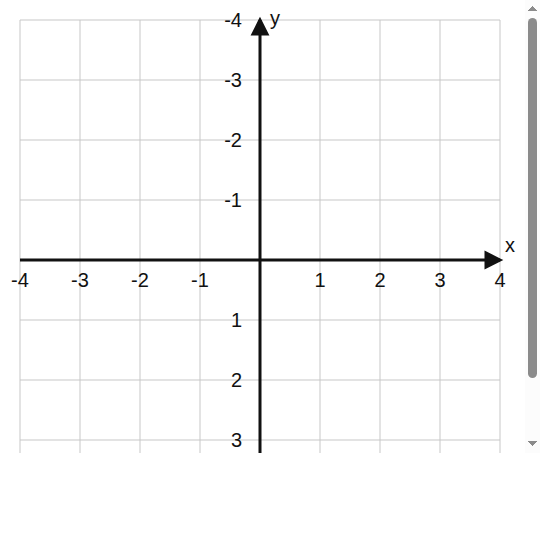
\includegraphics[width=0.88\linewidth]{web-diagrams/coord-grid.png}}
\task {Draw \mbox{$y=3^{x}-5$}. Mark the horizontal asymptote. \\[0.4em] 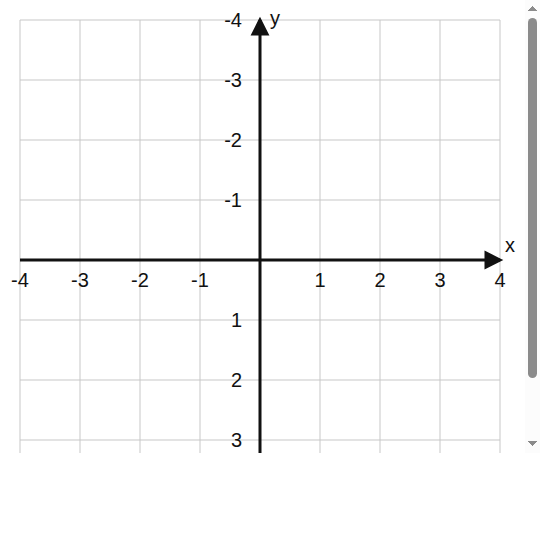
\includegraphics[width=0.88\linewidth]{web-diagrams/coord-grid.png}}
\task {Draw \mbox{$y=2^{x-2}+1$}. Mark the horizontal asymptote. \\[0.4em] 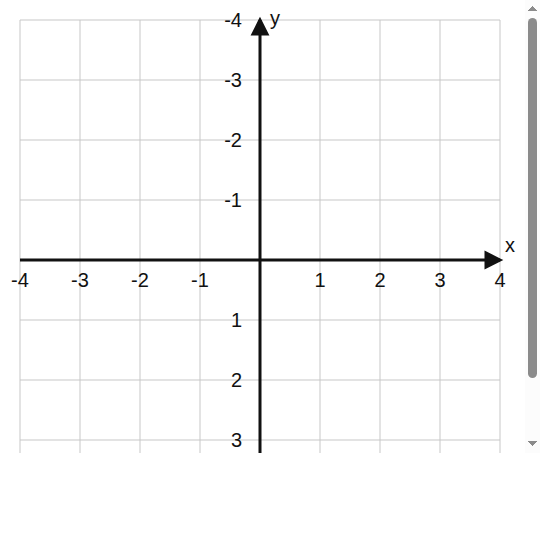
\includegraphics[width=0.88\linewidth]{web-diagrams/coord-grid.png}}
\task {Draw \mbox{$y=2^{x+1}-3$}. Mark the horizontal asymptote. \\[0.4em] 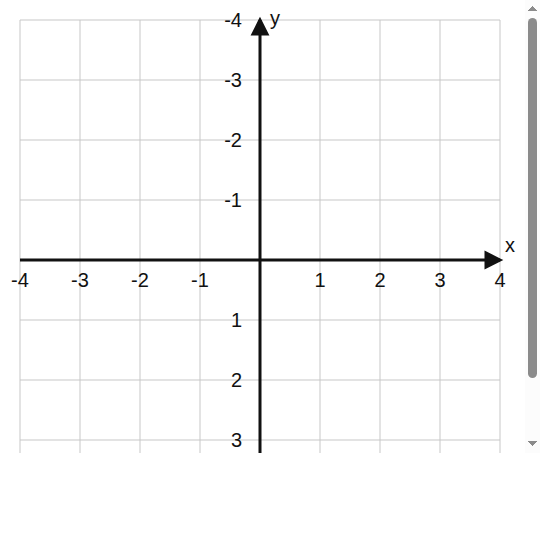
\includegraphics[width=0.88\linewidth]{web-diagrams/coord-grid.png}}
\task {Draw \mbox{$y=4\left(\frac{1}{2}\right)^x+1$}. Mark the horizontal asymptote. \\[0.4em] 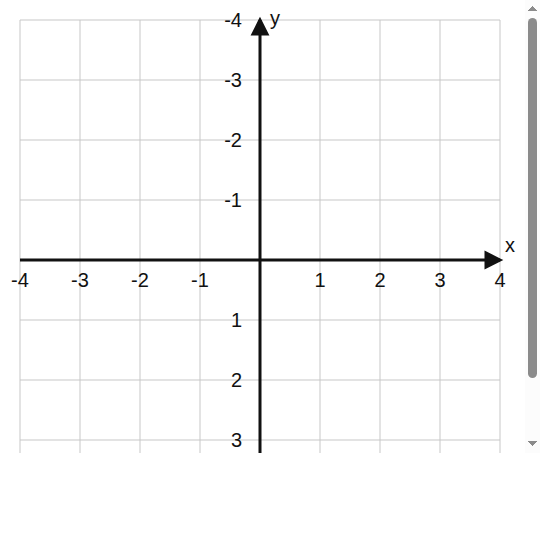
\includegraphics[width=0.88\linewidth]{web-diagrams/coord-grid.png}}
\task {Draw \mbox{$y=3\left(\frac{1}{3}\right)^x-2$}. Mark the horizontal asymptote. \\[0.4em] 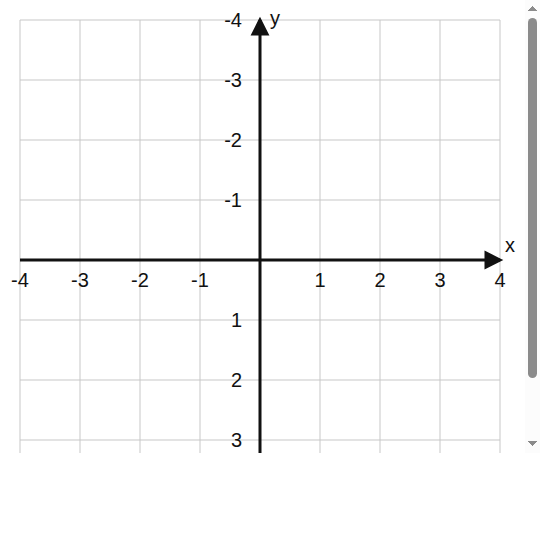
\includegraphics[width=0.88\linewidth]{web-diagrams/coord-grid.png}}
\task {Draw \mbox{$y=2\cdot 2^x-1$}. Mark the horizontal asymptote. \\[0.4em] 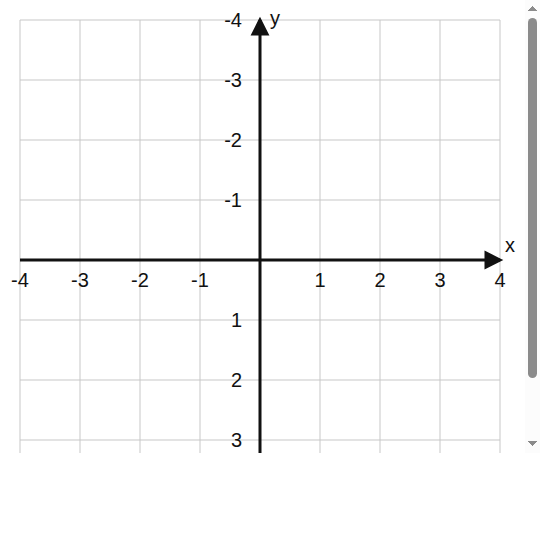
\includegraphics[width=0.88\linewidth]{web-diagrams/coord-grid.png}}
\task {Draw \mbox{$y=\frac{1}{2}\cdot 3^x+2$}. Mark the horizontal asymptote. \\[0.4em] 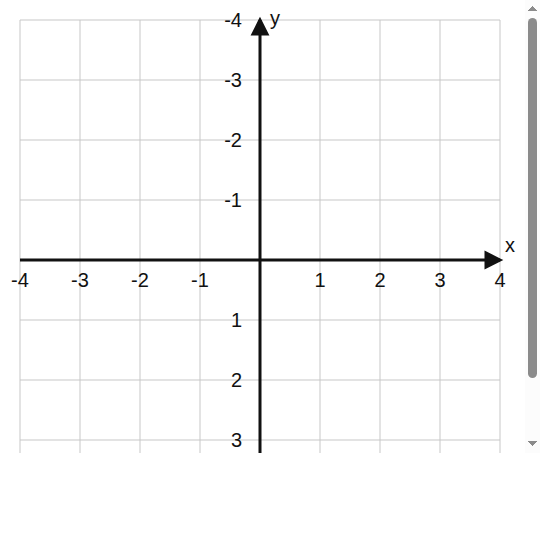
\includegraphics[width=0.88\linewidth]{web-diagrams/coord-grid.png}}
\task {Draw \mbox{$y=5\left(\frac{1}{2}\right)^{x-1}$}. State whether the graph is growth or decay. \\[0.4em] 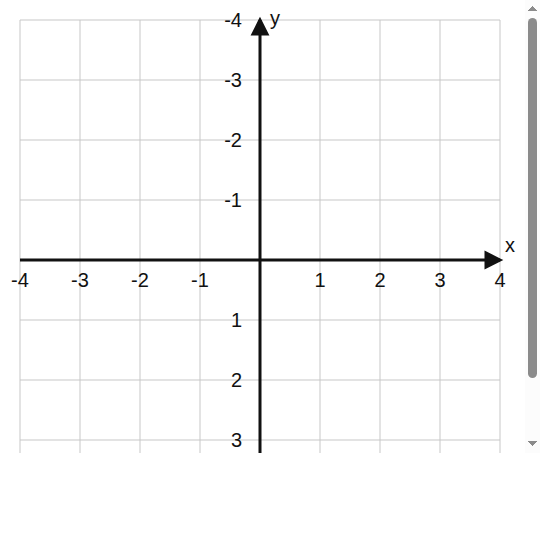
\includegraphics[width=0.88\linewidth]{web-diagrams/coord-grid.png}}
\task {Draw \mbox{$y=2\left(\frac{1}{3}\right)^{x+1}+1$}. State whether the graph is growth or decay. \\[0.4em] 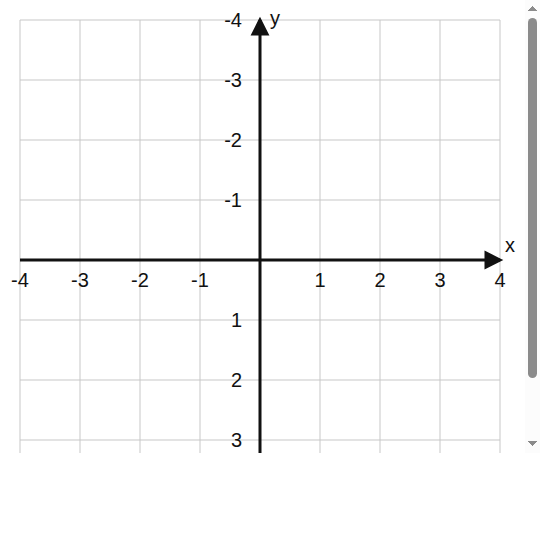
\includegraphics[width=0.88\linewidth]{web-diagrams/coord-grid.png}}
\task {Draw \mbox{$y=3^{x-1}-4$}. Mark the horizontal asymptote and the \mbox{$y$}-intercept. \\[0.4em] 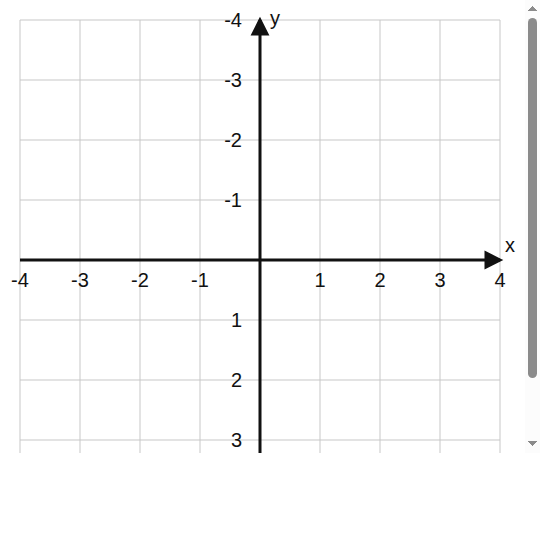
\includegraphics[width=0.88\linewidth]{web-diagrams/coord-grid.png}}
\task {Draw \mbox{$y=2^{x+2}+2$}. Mark the horizontal asymptote and the \mbox{$y$}-intercept. \\[0.4em] 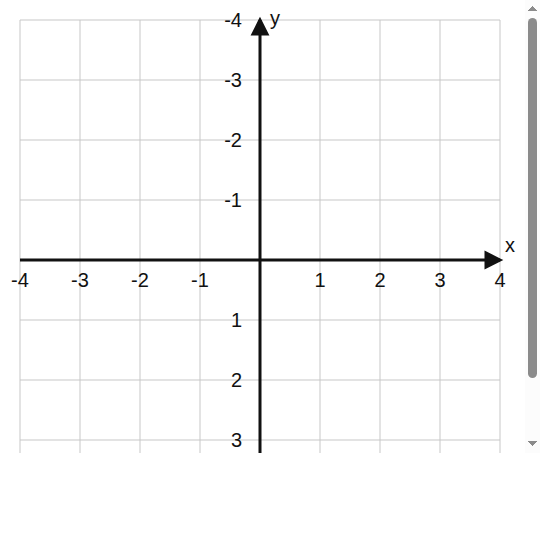
\includegraphics[width=0.88\linewidth]{web-diagrams/coord-grid.png}}
\task {Draw \mbox{$y=6\left(\frac{1}{2}\right)^x-3$}. Mark the horizontal asymptote and the \mbox{$y$}-intercept. \\[0.4em] 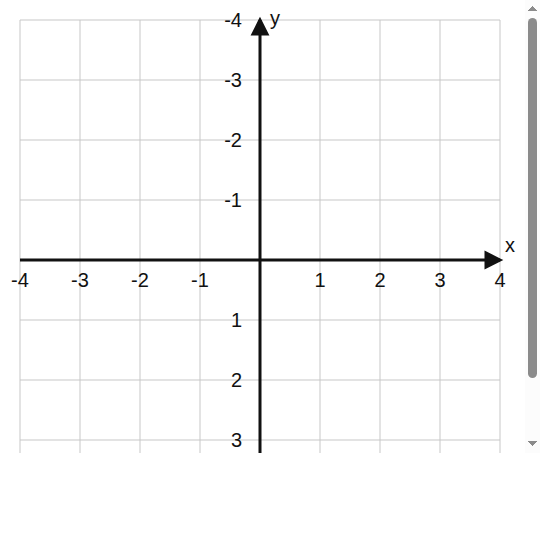
\includegraphics[width=0.88\linewidth]{web-diagrams/coord-grid.png}}
\task {Draw \mbox{$y=2\cdot 4^x+1$}. Mark the horizontal asymptote and the \mbox{$y$}-intercept. \\[0.4em] 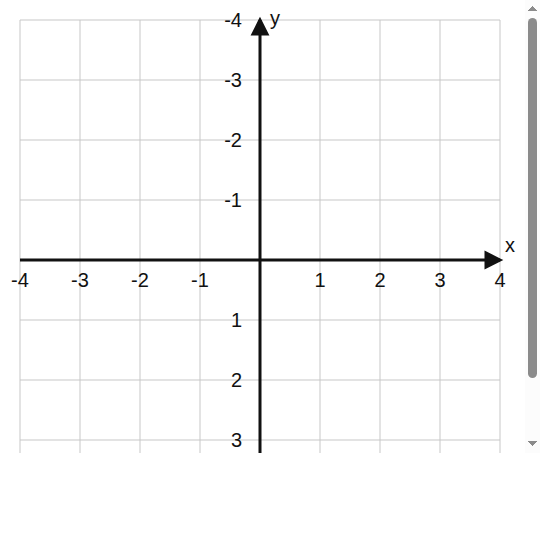
\includegraphics[width=0.88\linewidth]{web-diagrams/coord-grid.png}}
\task {Draw \mbox{$y=\frac{1}{4}\cdot 2^x-2$}. Mark the horizontal asymptote and the \mbox{$y$}-intercept. \\[0.4em] 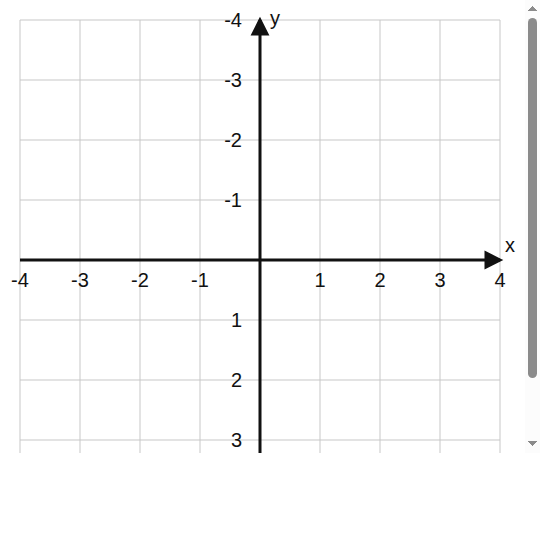
\includegraphics[width=0.88\linewidth]{web-diagrams/coord-grid.png}}
\task {Draw \mbox{$y=4\left(\frac{1}{2}\right)^x+3$}. Mark the horizontal asymptote and the \mbox{$y$}-intercept. \\[0.4em] 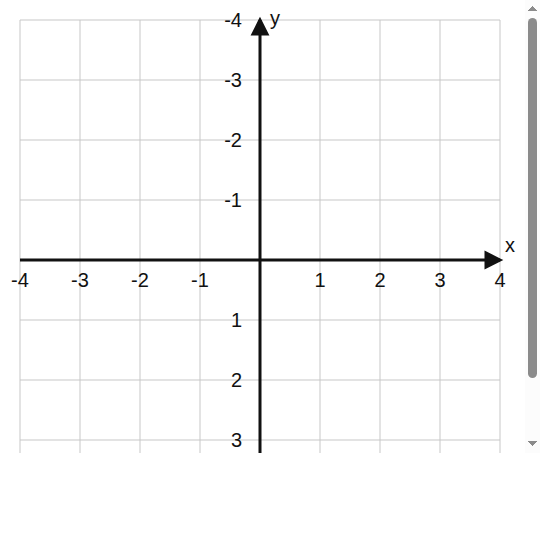
\includegraphics[width=0.88\linewidth]{web-diagrams/coord-grid.png}}
\end{tasks}

\end{document}
